\newcommand{\econtexRoot}{..}
\documentclass{beamer}\usepackage{dcolumn}
% \documentclass[aspectratio=169]{beamer}
\usepackage{verbatim}
\usepackage{cancel}
\usepackage{econtexShortcuts}
\usepackage{wasysym,ifthen,mathrsfs}
\usepackage[english]{babel}
\usepackage{color}
\usepackage[latin1]{inputenc}
\usepackage{booktabs,natbib}
\usepackage{tikz} 
\usetikzlibrary{tikzmark,fit,shapes.geometric}
\usetikzlibrary{tikzmark,calc,arrows,shapes,decorations.pathreplacing}
\tikzset{every picture/.style={remember picture}}
% Resources that need to be accessible from various different locations

\providecommand{\YLevBF}{\ensuremath{\mathbf{Y}}}
\renewcommand{\pDies}{\ensuremath{\mathsf{d}}}
%\renewcommand{\PDies}{\ensuremath{\mathsf{D}}}
%\renewcommand{\PLives}{\ensuremath{(1-\mathsf{D})}}

\providecommand{\aggrSavingRuleCoeff}{\ensuremath{\kappa}}
\providecommand{\stnRatio}{\ensuremath{\tau}}

\newcommand{\TabsDir}{\econtexRoot/Tables}\newcommand{\Calibration}{\econtexRoot/Calibration}
\newcommand{\W}{\mathcal{W}}            % Include or exclude aggregate wage in individual problem - to include, should be \newcommand{\W}{W}

\provideboolean{Depreciation}
\setboolean{Depreciation}{true}
%\setboolean{Depreciation}{false}
\provideboolean{MicroDepr}
\setboolean{MicroDepr}{true}
%\setboolean{Depreciation}{false}
\newcommand{\ifDepr}{\ifthenelse{\boolean{Depreciation}}}
\newcommand{\MicroDepr}{\ifthenelse{\boolean{MicroDepr}}}

\newcommand{\RBet}{\mathbf{R}} % Bold  version is between-period rate; \mathcal version is within
\newcommand{\rBet}{\mathbf{r}} % Bold  version is between-period rate; \mathcal version is within
\newcommand{\RIn}{\mathcal{R}}
\newcommand{\rIn}{r}

\provideboolean{Growth}
\setboolean{Growth}{true}
\setboolean{Growth}{false}
\newcommand{\ifGG}{\ifthenelse{\boolean{Growth}}}  % Switch for whether to include productivity growth in formulae; useful for programming/debugging

\provideboolean{numSwitch}     % Switch that suppresses eqn numbers on slides but not in text
\setboolean{numSwitch}{true}   % Set to true  at beginning of text
%\setboolean{numSwitch}{false} % Set to false at beginning of slides
\providecommand{\ifnumSw}{\ifthenelse{\boolean{numSwitch}}{}{\nonumber}}

\provideboolean{Slides}
\setboolean{Slides}{false}
\newcommand{\ifslides}{\ifthenelse{\boolean{Slides}}}

\provideboolean{ZeroProb}
\setboolean{ZeroProb}{false}
\setboolean{ZeroProb}{true}
\newcommand{\ifZero}{\ifthenelse{\boolean{ZeroProb}}}

\provideboolean{DocVersion} % If true, produce an elaborate version of the document that contains all formulae used in the software
\setboolean{DocVersion}{false}
\setboolean{DocVersion}{true}
%\providecommand{\ifDoc}{\ifthenelse{\boolean{DocVersion}}}
\providecommand{\ifDoc}{\marginpar{\tiny{DocAndNodocVersions}}\emph}

% ExtraExplain toggles whether to include the explanation for why we can't assume \bar{\ell}=\ell
\provideboolean{ExtraExplain}
\setboolean{ExtraExplain}{false}
%\setboolean{ExtraExplain}{true}
\newcommand{\ifExplain}{\ifthenelse{\boolean{ExtraExplain}}}

\provideboolean{ShowStickyE}
\setboolean{ShowStickyE}{true}
\setboolean{ShowStickyE}{false}
\newcommand{\StickyE}{\ifthenelse{\boolean{ShowStickyE}}}

\newcommand{\eq}{\econtexRoot/Equations}
\newcommand{\EqnDir}{\econtexRoot/Equations}

\newcommand{\fm}{frictionless-$\mathbf{m}$ }
\newcommand{\sm}{sticky-$\mathbf{m}$ }

\newcommand{\ParmDir}{\econtexRoot/Calibration}
\newcommand{\TablesDir}{\econtexRoot/Tables}
\newcommand{\DirCampManVsStickyE}{\econtexRoot/Empirical/US/Results/LaTeX/tables}
\providecommand{\perc}[1]{\widetilde{#1}}

\pdfmapfile{+sansmathaccent.map}

\definecolor{myRed}{rgb}{0.8,0,0}
\definecolor{jirkasblue}{rgb}{0.2,0.2,0.7}
\definecolor{jirkasred}{rgb}{0.9,0,0}
\definecolor{LightCyan}{rgb}{0.88,1,1}
\definecolor{SlideNavy}{rgb}{0,0,0.54}
\definecolor{StataDarkBlue}{rgb}{0,0,0.835}
\definecolor{Pink}{rgb}{1,0.8,0.8}

\newcolumntype{g}{>{\columncolor{Pink}}d{3}}
\newcommand{\jemph}[1]{{\color{StataDarkBlue}#1}}
\newcommand{\jbemph}[1]{\textbf{\color{SlideNavy}#1}}
\newcommand{\var}{\ensuremath{\text{var}}}

\mode<presentation>
{
  \usetheme{default} % Singapore % Montpellier
  \setbeamercovered{transparent}
}

% if this is on, bullets are shown step by step
%\beamerdefaultoverlayspecification{<+->}

%\setbeamertemplate{navigation symbols}{}  % Take away navigation symbols

\providecommand{\W}{\mathcal{W}}            % Include or exclude aggregate wage in individual problem - to include, should be
\providecommand{\perc}[1]{\widetilde{#1}}

\provideboolean{Depreciation}
\setboolean{Depreciation}{true}
%\setboolean{Depreciation}{false}
\provideboolean{MicroDepr}
\setboolean{MicroDepr}{true}
%\setboolean{Depreciation}{false}
\providecommand{\ifDepr}{\ifthenelse{\boolean{Depreciation}}}
\providecommand{\MicroDepr}{\ifthenelse{\boolean{MicroDepr}}}

\ifDepr{
\providecommand{\RBet}{\mathbf{R}} % Bold  version is between-period rate; \mathcal version is within
\providecommand{\rBet}{\mathbf{r}} % Bold  version is between-period rate; \mathcal version is within
\providecommand{\RIn}{\mathcal{R}}
\providecommand{\rIn}{r}
}{
\providecommand{\RBet}{R} % Bold  version is between-period rate; \mathcal version is within
\providecommand{\rBet}{r} % Bold  version is between-period rate; \mathcal version is within
\providecommand{\RIn}{R}
\providecommand{\rIn}{r}
\providecommand{\rNet}{\mathfrak{r}} % For defining consumption Euler equation
}

\provideboolean{Growth}
\setboolean{Growth}{true}
\setboolean{Growth}{false}
\providecommand{\ifGG}{\ifthenelse{\boolean{Growth}}}  % Switch for whether to include productivity growth in formulae; useful for programming/debugging

\provideboolean{numSwitch}     % Switch that suppresses eqn numbers on slides but not in text
\setboolean{numSwitch}{true}   % Set to true  at beginning of text
%\setboolean{numSwitch}{false} % Set to false at beginning of slides
\providecommand{\ifnumSw}{\ifthenelse{\boolean{numSwitch}}{}{\nonumber}}

\provideboolean{Slides}
\setboolean{Slides}{false}
\providecommand{\ifslides}{\ifthenelse{\boolean{Slides}}}

\provideboolean{ZeroProb}
\setboolean{ZeroProb}{false}
\setboolean{ZeroProb}{true}
\providecommand{\ifZero}{\ifthenelse{\boolean{ZeroProb}}}

\provideboolean{DocVersion} % If true, produce an elaborate version of the document that contains all formulae used in the software
\setboolean{DocVersion}{false}
\setboolean{DocVersion}{true}
\providecommand{\ifDoc}{\ifthenelse{\boolean{DocVersion}}}

% ExtraExplain toggles whether to include the explanation for why we can't assume \bar{\ell}=\ell
\provideboolean{ExtraExplain}
\setboolean{ExtraExplain}{true}
\providecommand{\ifExplain}{\ifthenelse{\boolean{ExtraExplain}}}

\provideboolean{ShowStickyE}
\setboolean{ShowStickyE}{true}
\setboolean{ShowStickyE}{false}
\providecommand{\StickyE}{\ifthenelse{\boolean{ShowStickyE}}}

\providecommand{\econtexRoot}{.}
\providecommand{\eq}{\econtexRoot/Equations}

\providecommand{\fm}{frictionless-$\mathbf{m}$ }
\providecommand{\sm}{sticky-$\mathbf{m}$ }

\providecommand{\ParmDir}{\econtexRoot/Calibration/Parameters}
\providecommand{\TablesDir}{\TabsDir}
%\providecommand{\ParmDir}{C:/Jirka/Research/stickyConsumptionUS/Nov26_07/cAndCwithStickyEArchive/Calibration/Parameters}
%\providecommand{\TablesDir}{C:/Jirka/Research/stickyConsumptionUS/Nov26_07/cAndCwithStickyEArchive/Tables}

%\input EconDocStart
%\input PDFDocStart
\mode<presentation>
{
  \usetheme{Madrid}
  % or ...

  \setbeamercovered{transparent}
  % or whatever (possibly just delete it)
}
\definecolor{jirkasred}{rgb}{0.9,0,0}
\definecolor{jirkasblue}{rgb}{0.2,0.2,0.7}
\providecommand{\jemph}[1]{{\color{jirkasblue}#1}}
\def\newblock{\hskip .11em plus .33em minus .07em}

\newcolumntype{d}[1]{D{.}{.}{#1}}

\usepackage[latin1]{inputenc}
% or whatever

\beamertemplatenavigationsymbolsempty

\title[]{Sticky Expectations and Consumption Dynamics}

\author[]{Christopher D. Carroll \and Edmund Crawley \and Jiri Slacalek \and Kiichi Tokuoka \and Matthew N. White}

%\institute % (optional, but mostly needed)
%{
%Board of Governors of the Federal Reserve System
%}
% - Use the \inst command only if there are several affiliations.
% - Keep it simple, no one is interested in your street address.
%\institute{
%  \inst{1} Johns Hopkins and NBER, \texttt{ccarroll@jhu.edu} %\\ \texttt{http://www.econ.jhu.edu/people/ccarroll/}
%  \and
%  \inst{2} Johns Hopkins,  \texttt{ecrawle2@jhu.edu} %\\ \texttt{http://www.slacalek.com/}
%  \and
%  \inst{3} European Central Bank,  \texttt{jiri.slacalek@ecb.int} %\\ \texttt{http://www.slacalek.com/}
%  \and
%  \inst{4} MoF Japan,  \texttt{kiichi.tokuoka@mof.go.jp}
%  \and
% \inst{5} University of Delaware,  \texttt{mnwecon@udel.edu}\\
%  }
\date[]{CEBRA Annual Meeting, New York, July 2019 % venue
}

\begin{document}

\newcolumntype{d}[1]{D{.}{.}{#1}}
\def\newblock{\hskip .11em plus .33em minus .07em}

\begin{frame}
  \titlepage
\end{frame}

%\section{Consumption: Micro Vs Macro}
%\subsection{Habits?  No!  It's Inattention}
\begin{frame}
\frametitle{Consumption Dynamics: Macro vs Micro}
Macro
\begin{itemize}
	\item \textit{Aggregate} consumption exhibits \textbf{`excess\tikz[baseline]{\node(excess){}} smoothness'}
\end{itemize}
Micro
\begin{itemize}
	\item \textit{Idiosyncratic} consumption does not \tikz[baseline]{\node(idio){}}
\end{itemize}
\bigskip
\only<1-3>{
	\textcolor{white}{This paper}
	\begin{itemize}
		\item[]
		\begin{itemize}
			\item[]
			\item[]
			\item[]
		\end{itemize}
	\end{itemize}
}
	\only<2->{
	\begin{tikzpicture}[remember picture,overlay]
	\node (excessa)  at ([shift={(0,0.3)}]excess) {};
	\node (excessb)  at ([shift={(0,1)}]excessa) {};
	\draw[blue,thick,->] (excessa)  to [in=270,out=90] (excessb) node[anchor=south,text = blue] { Modeling response: `habits'};
	\end{tikzpicture}
}
	\only<3->{
	\begin{tikzpicture}[remember picture,overlay]
	\node (idioa)  at ([shift={(0,0.1)}]idio) {};
	\node (idiob)  at ([shift={(0.8,0.0)}]idioa) {};
	\draw[blue,thick,->] (idioa)  to [in=180,out=0] (idiob) node[anchor=west,text = blue] {Habits strongly rejected};
	\end{tikzpicture}
}
\only<4->{
This paper
	\begin{itemize}
		\item Builds a model that reconciles these empirical facts
		\begin{itemize}
			\item Sticky Expectations replace habits
			\item Tractable
			\item Quantitatively plausible (both micro and macro)
		\end{itemize}
	\end{itemize}
}

\end{frame}
\begin{comment}
\begin{frame}
\frametitle{Consumption Dynamics: Macro vs Micro}
%  \jbemph{\large C growth persistent in macro but not micro data}
\begin{block}{Macro: Representative Agent Models}
	\begin{itemize}
		\item  Basic Theory: C responds instantly, completely to shock
		\item Evidence: Consumption is too smooth {\scriptsize (Campbell {\&} Deaton, 1989)}
		\item Solution: \jbemph{``Habits'' parameter $\chi^{\text{Macro}}\approx 0.6$--$0.8$}\\
		\centerline{       $\Delta \log \mathbf{C}_{t+1} = \varsigma + \chi \Delta \log \mathbf{C}_t +\epsilon $}
	\end{itemize}
\end{block}

\begin{block}{Micro: Heterogeneous Agent Models}
	\begin{itemize}
		\item  \jbemph{Uninsurable risk is essential, changes everything}
		\item Var of micro income shocks much larger than of macro shocks:\\
		\centerline{    \%jemph{var$(\Delta \log \pLevBF) \approx  100\times$var($\Delta \log \PLevBF$)}}
		\item Evidence: \jbemph{``Habits'' parameter $\chi^{\text{Micro}}\approx 0.0$--$0.1$}
	\end{itemize}
\end{block}
\end{frame}
\end{comment}

\begin{frame}
  \frametitle{Excess Smoothness: Macro vs Micro}
Estimate $\chi$ in \\ 
\centering
$ \Delta \log \mathbf{C}_{t+1} = \varsigma + \chi \Delta \log \mathbf{C}_t +\epsilon $\\
\bigskip
597 estimates of $\chi$ in \cite*{havranek:metaHabits}
	\begin{columns}
	\column{0.7\linewidth}
	\centering
\begin{figure}
\begin{center}
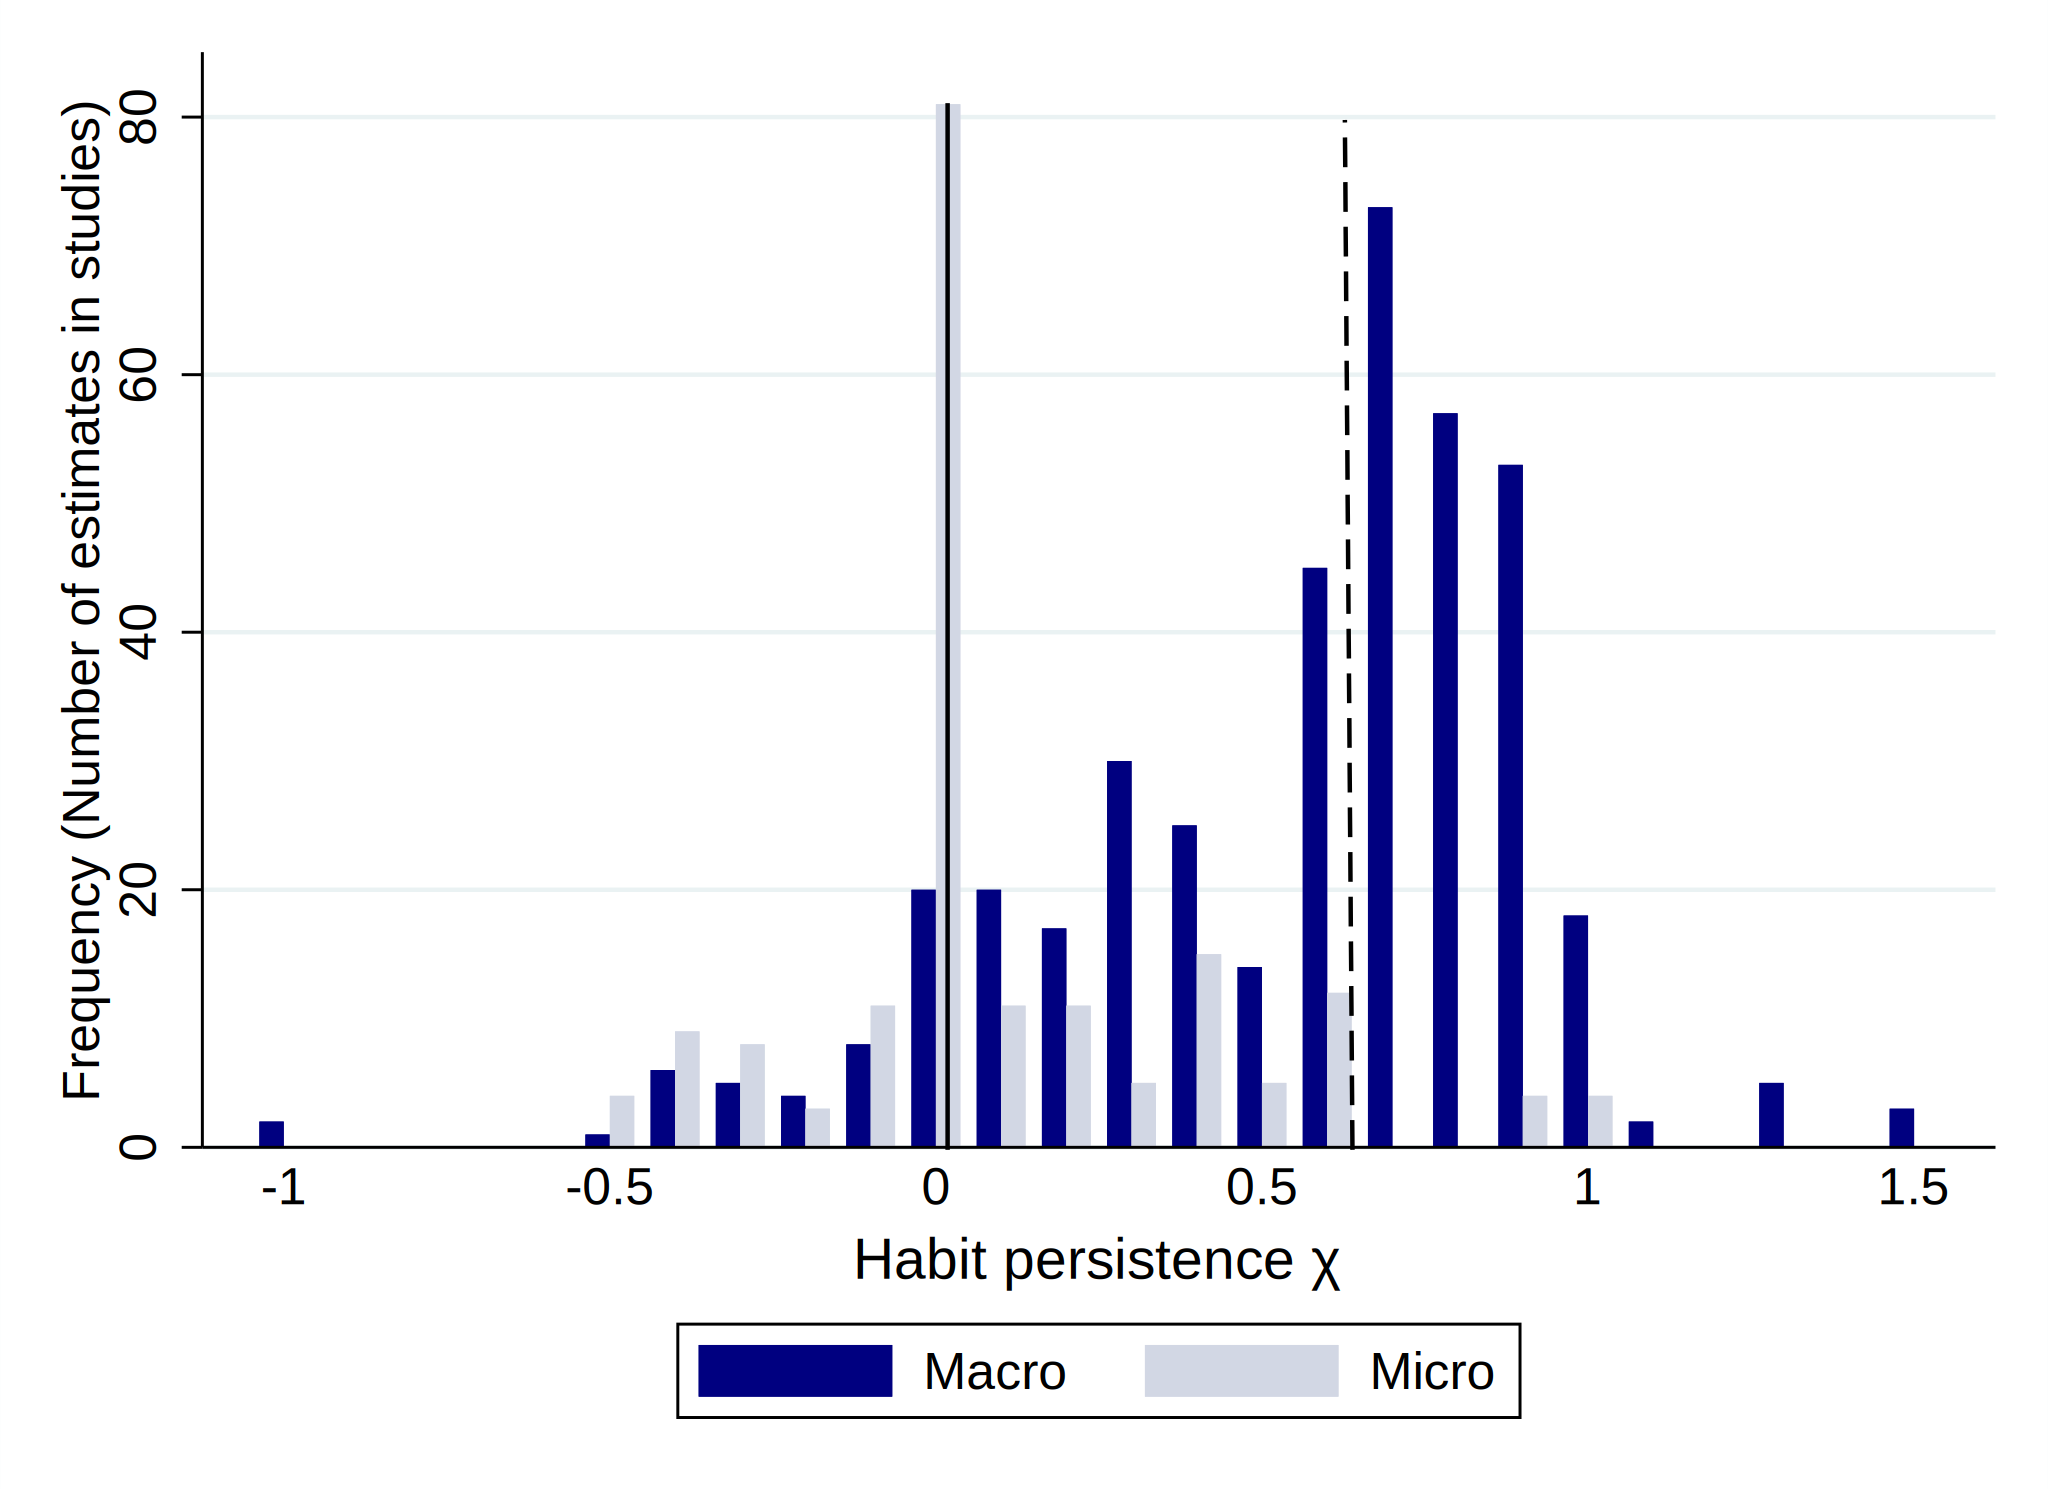
\includegraphics[width=.90\textwidth]{../Figures/microMacroMetaHistogram}
\end{center}
\end{figure}
\column{0.3\linewidth}
$\chi^{\text{Macro}}\approx 0.6$ \\
\bigskip
$\chi^{\text{Micro}}\approx 0.1$ \\
\end{columns}

\end{frame}

\begin{frame}
\frametitle{Claim: It's Not Habits, It's (Macro) Inattention! }
\jbemph{\large Our Income Process}
\begin{itemize}
\item   Idiosyncratic Component: Perfectly Observed
\item   \jbemph{Aggregate Component: Stochastically Observed}\\
  \begin{itemize}
\item Updating \`a la \cite{calvoPrices}
  \end{itemize}

\end{itemize}
\begin{block}{ Advantages}
\begin{itemize}
\item Resolves macro/micro habits dissonance
\item Simple to apply in heterogenous agent settings
  \begin{itemize}
	\item e.g. \cite{arsInvestmentInattention}
\end{itemize}
\end{itemize}
\end{block}

\end{frame}

\begin{frame}
\frametitle{Why Macro Inattention Is Plausible}

\begin{block}{\textbf{Idiosyncratic Variability Is $\sim$ 100$\times$ Bigger}}
\begin{itemize}
\item  If Same Specification Estimated on Micro vs Macro Data
\item  Pervasive Lesson of All Micro Data
\end{itemize}
\end{block}

\begin{block}{\textbf{Utility Cost of Inattention Small}}
\begin{itemize}
\item  Micro: Critical (and Easy) To Notice You're Unemployed
% \item Unlike \cite{pischkeMicroMacro}
\item  Macro: {\it Not} Critical To Instantly Notice If U $\uparrow$
\end{itemize}
\end{block}
\end{frame}

%\section{\href{http://www.econ2.jhu.edu/people/ccarroll/public/LectureNotes/Consumption/StickyExpectationsC/}{Toy Model}}
%\subsection{Toy Model}
\begin{frame}
\frametitle{Quadratic Utility `Toy Model'}

\begin{block}{\cite{hallRandomWalk} Random Walk}
\phantom{.}
\begin{itemize}
\item \%jemph{Total Wealth} (Human$\,+\,$Nonhuman):\\
\begin{center}
{$\wAllLev_{t+1} = (\wAllLev_{t}-\cLevBF_{t})\Rfree+\zeta_{t+1}$}
\end{center}
\item \%jemph{Euler Equation}: \\
\begin{center}
{$\uFunc^{\prime}(\cLevBF_{t}) = \Rfree\beta \Ex_{t}[\uFunc^{\prime}(\cLevBF_{t+1})]$}
\end{center}
\item $\Rightarrow$ \%jemph{Random Walk} (for $\Rfree\beta=1$): \\
\begin{center}
{$\Delta \cLevBF_{t+1} = \epsilon_{t+1}$}
\end{center}
\item \%jemph{Expected Wealth}: \\
\begin{center}
{$\wAllLev_{t} = \Ex_{t}[\wAllLev_{t+1}] = \Ex_{t}[\wAllLev_{t+2}] = \dots$}
\end{center}
\end{itemize}
\end{block}

\end{frame}

\begin{frame}
\frametitle{Sticky Expectations---Individual $\mathbf{c}$}

\begin{itemize}
\item
Consumer who happens to update at $t$ and $t+n$
\begin{eqnarray*}
\ifnumSw         \cLevBF_{t  } & = & (\rfree/\Rfree)\wAllLev_{t} \label{eq:ct}
\ifnumSw \\      \cLevBF_{t+1} & = & (\rfree/\Rfree)\perc{\wAllLev}_{t+1} = (\rfree/\Rfree)     \wAllLev _{t} = \cLevBF_{t}
%\ifnumSw \\      \cLevBF_{t+2} & = & (\rfree/\Rfree)\perc{\wAllLev}_{t+2} = (\rfree/\Rfree)     \wAllLev _{t} = \cLevBF_{t}
\ifnumSw \\               \vdots  &  & \vdots \nonumber
\ifnumSw \\        \cLevBF_{t+n-1} & = & \cLevBF_{t}
\label{eq:ctpn}
\end{eqnarray*}

\item
Implies that $\Delta^{n} \wAllLev_{t+n} \equiv \wAllLev_{t+n}-\wAllLev_{t}$ is white noise

\item So \jbemph{individual} $\mathbf{c}$ is RW across updating periods:
\begin{eqnarray*}
\ifnumSw  \mathbf{c}_{t+n}-\mathbf{c}_{t} & = & (\rfree/\Rfree)\underbrace{(\wAllLev_{t+n}-\wAllLev_{t}) }_{\Delta^{n} \wAllLev_{t+n}}
\end{eqnarray*}
%\item \jbemph{No persistence in individual c growth}
\end{itemize}
\end{frame}

\begin{frame}
\frametitle{Sticky Expectations---Aggregate $\mathbf{C}$}

\begin{itemize}
\setlength{\itemsep}{2mm}
\item Aggregate: $\CLevBF_{t} = \int_{0}^{1} \cLevBF_{t,i}\,\text{d}i$
\item \jbemph{\cite{calvoPrices}-Type Updating of Expectations:}
\begin{itemize}
\item Probability $\Pi = 0.25$ (per quarter)
%\item NOT Muth/Lucas/Pischke/Reis signal extraction
\end{itemize}

\item Economy composed of many sticky-$\Ex$ consumers:
\begin{eqnarray*}
 \CLevBF_{t+1} & = & (1-\Pi) \underbrace{\CLevBF^{\cancel{{\pi}}}_{t+1}}_{=\CLevBF_{t}} \label{eq:Ctp1} + \Pi \CLevBF^{{\pi}}_{t+1}
 \\
%\end{eqnarray*}
%\begin{eqnarray*}
  \Delta \mathbf{C}_{t+1} & \approx & \underbrace{(1-\Pi)}_{{}\equiv\chi=0.75} \Delta \mathbf{C}_{t} + \epsilon_{t+1}
\end{eqnarray*}
\item \jbemph{Substantial persistence ($\chi=0.75$) in aggregate C growth}
\end{itemize}
\end{frame}

\begin{frame}
\frametitle{One More Ingredient \dots}

\begin{itemize}
\setlength{\itemsep}{2mm}
\item[] \%jemph{Idiosyncratic shocks:} Frictionless observation
  \begin{itemize}
  \setlength{\itemsep}{1mm}
  \item I notice if I am fired, promoted, somebody steals my wallet
  \end{itemize}
\item[] \%jemph{Aggregate shocks:} Sticky observation
 \begin{itemize}
   \setlength{\itemsep}{1mm}
  \item May not instantly notice changes in aggregate productivity
  \end{itemize}
\end{itemize}
\bigskip
So...
\begin{itemize}
  \setlength{\itemsep}{1mm}
\item[]  \%jemph{Idiosyncratic $\Delta \mathbf{c}$}: dominated by frictionless dynamics
\end{itemize}
But law of large numbers $\Rightarrow$ idiosyncratic part vanishes
\begin{itemize}
\item[]  \%jemph{Aggregate     $\Delta \mathbf{C}$}: highly serially correlated
\end{itemize}

\end{frame}

%\section{The Real Model}
%\subsection{Frictionless Setup}
\begin{frame}
\frametitle{Full Model}

\begin{block}{Partial Equilibrium/Small Open Economy}
\begin{itemize}
\item  CRRA Utility
\item  Idiosyncratic Shocks Calibrated From Micro Data
\item  Aggregate Shocks Calibrated From Macro Data
\item Markov Process (Discrete RW) for Agg. Income Growth
  \begin{itemize}
  \item Handles changing growth `eras'
  \end{itemize}
\item  Liquidity Constraint
\item  Mildly Impatient Consumers
\item  \cite{blanchardFinite} Mortality and Insurance
\end{itemize}
\end{block}

\end{frame}

\begin{frame}
\frametitle{Solving the Model}

All results are generated using the open-source Econ-ARK toolkit:
\bi
\item \url{http://econ-ark.org}
\ei

\end{frame}

\begin{frame}
\frametitle{Income Process}

\begin{itemize}
\item  Individual's labor productivity is
$$
\pmb{\ell}_{t,i} = \overbrace{\theta_{t,i}\Theta_{t}}^{\equiv\,\pmb{\theta}_{t,i}}\overbrace{{p}_{t,i} {P}_{t}}^{\equiv\, \pLev_{t,i}}
$$

\item  Idiosyncratic and aggregate $p$ evolve according to
\begin{eqnarray*}
{{p}}_{t+1,i} & =&  \phantom{\%jemph{\PtyGro}_{t+1}}{{p}}_{t,i} \psi_{t+1,i}  \\
 {P}_{t+1\phantom{,i}} & =&  \%jemph{\PtyGro}_{t+1} {P}_{t\phantom{,i}}\Psi_{t+1}
\end{eqnarray*}

%\item  $\Ex_{t}[\theta_{t+n}]=\Ex_{t}[\Theta_{t+n}]=\Ex_{t}[\pShk_{t+n}]=\Ex_{t}[\PShk_{t+n}]=1\quad\forall~n>0$

  \item \jbemph{$\PtyGro$ is Markov `underlying' aggregate pty growth}
    \begin{itemize}
    \setlength{\itemsep}{1mm}
    \item Discrete (bounded) random walk
    \item Calibrated to match postwar US pty growth variation
    \item Generates predictability in income growth (for IV regressions)
    \end{itemize}
  \end{itemize}
\end{frame}

%\subsection{Sticky Expectations}
\begin{frame}
\frametitle{Sticky Expectations about Aggregate Income}

\jbemph{\large Calvo Updating of Perceptions of Aggregate Shocks}\\
\bi
\item {\it True} Permanent income: ${P}_{t+1} =  \PtyGro_{t+1} {P}_{t}\Psi_{t+1}$\\
\item Tilde ($\perc{P}$) denotes perceived variables
\item \%jemph{Perception for consumer who has not updated for $n$ periods:}
$$
  \perc{P}_{t,i}=\Ex_{t-n}\big[P_t\big\vert\Omega_{t-n}\big]=\Phi_{t-n}^nP_{t-n}
$$
because $\Phi$ is random walk
\ei
\bigskip  
\%jemph{\textbf{Key Assumption:}}\\
\begin{itemize}
	\item  People act as if their perceptions about aggregate state $\{\perc{P}_{t,i},\perc{\PtyGro}_{t,i}\}$
	are the true aggregate state $\{P_t,\PtyGro_t\}$
	\item[] $\implies$ Model solution is \textit{exactly} the same as the frictionless model
\end{itemize}
\end{frame}

\begin{comment}
\begin{frame}
\frametitle{Sticky Expectations about Aggregate Income}

\jbemph{\large Sequence Within Period}\\
\begin{enumerate}
\setlength{\itemsep}{2mm}
\item Income shocks are realized and every individual sees her true income, $\mathbf{y}$ and market resources, $\mathbf{m}$

\item Updating shocks realized: $i$ observes true $P_t, \PtyGro_t$ w/ prob $\Pi$

\item Consumes based on her perception of the aggregate state\\
\bigskip
  \%jemph{\textbf{Key Assumption:}}\\
    \begin{itemize}
    \item  People act as if their perceptions about aggregate state $\{\perc{P}_{t,i},\perc{\PtyGro}_{t,i}\}$
are the true aggregate state $\{P_t,\PtyGro_t\}$
\item[] $\implies$ Model solution is \textit{exactly} the same as the frictionless model
    \end{itemize}

\end{enumerate}

\end{frame}
\end{comment}

\begin{frame}
\frametitle{Key Parameter Values}
\label{key_parameters}
%\ptsize{9}
\small
\begin{center}
	\begin{tabular}{cd{5}l}  
		\\ \toprule  
		\multicolumn{3}{c}{ \textbf{Preference Parameters} }  
		\\ $\rho$ & 2 & Coefficient of Relative Risk Aversion 
		\\ $\beta$ &  0.970 & Discount Factor (SOE Model) 
		\\ $\Pi$                    & 0.25  & Probability of Updating Expectations (if Sticky) 
		\\ ${K}/{K}^{\kapShare}$ & 12.0 & SS Capital to Output Ratio 
		\\ \midrule  
		\multicolumn{3}{c}{ \textbf{Shock Parameters} }  
		\\ $\sigma_{\theta}^{2}$    & 0.120     & Variance Idiosyncratic Tran Shocks (=$4 \times$ Annual) 
		\\ $\sigma_{\psi}^{2}$      &0.003      & Variance Idiosyncratic Perm Shocks (=$\frac{1}{4} \times$ Annual) 
		\\ $\sigma_{\Theta}^{2}$ & 0.00001 & Variance Aggregate Transitory Shocks 
		\\ $\sigma_{\Psi}^{2}$ & 0.00004 & Variance Aggregate Permanent Shocks 
		\\ $\wp$                    & 0.050  & Probability of Unemployment Spell 
		\\ $\PDies$             & 0.005  & Probability of Mortality 
		\\ \bottomrule  
	\end{tabular}  
\end{center} 

\hyperlink{calibration1}{\beamerbutton{Full Calibration}}

\end{frame}

\begin{frame}
\frametitle{Regressions on Simulated and Actual Data}
\jbemph{\cite{dynanHabits}/\cite{som07} Specification:}
$$
 \Delta \log \mathbf{C}_{t+1} \approx  \varsigma +\chi \Ex[ \Delta \log \mathbf{C}_{t}] + \eta \Ex[\Delta \log \mathbf{Y}_{t+1}]+\alpha A_{t}   +\epsilon_{t+1}
$$
\vspace*{-0.5cm}
\begin{itemize}
\setlength{\itemsep}{2mm}
\item \jbemph{$\chi$: Extent of habits}\\
\%jemph{Data: Micro:} $\chi^{\text{Micro}} = 0.1$ (EER 2017 paper)\\
\hspace*{1.1cm}\%jemph{Macro:} $\chi^{\text{Macro}} = 0.6$

\item  \jbemph{$\eta$: Fraction of Y going to `rule-of-thumb' C\,=\,Y types}\\
\%jemph{Data: Micro:} $0<\eta^{\text{Micro}} <1$ (Depends \dots)\\
\hspace*{1.1cm}\%jemph{Macro:} $\eta^{\text{Macro}} \approx 0.5$ (\cite{cmModel})

\item  \jbemph{$\alpha$: Precautionary saving (micro) or IES (Macro)}\\
\%jemph{Data: Micro:} $\alpha^{\text{Micro}}<0$ (\cite{zeldes:jpe})\\
\hspace*{1.1cm}\%jemph{Macro:} $\alpha^{\text{Macro}}<0$ (but small)\\
{[In GE $\rfree$ depends roughly linearly on $A$]}
\end{itemize}

\end{frame}

\begin{comment}
\begin{frame}
\frametitle{Micro vs Macro: Theory and Empirics}
\begin{eqnarray}
\ifnumSw\Delta \log \mathbf{C}_{t+1} & \approx & \varsigma+\chi \Delta \log \mathbf{C}_{t}+\eta \Ex_{t}[\Delta \log \mathbf{Y}_{t+1}]+\alpha A_{t}+\epsilon_{t+1} \nonumber
\end{eqnarray}

\begin{center}
\begin{tabular}{llccc}
\toprule
        &        & $\chi$       & $\eta$          & $\alpha$
\\ \midrule \multicolumn{2}{l}{Micro (Separable)}
\\    & Theory                 & $\approx 0  $      & $0 < \eta < 1 $ & $< 0$
\\        & Data                   & $\approx 0  $      & $0 < \eta < 1 $ & $< 0$
\\ \midrule \multicolumn{2}{l}{Macro}
\\ & Theory: Separable          & $\approx 0   $     & $\approx 0$           & $< 0$
\\ & Theory: CampMan            & $\approx 0   $     & $\approx 0.5$           & $< 0$
\\ & Theory: Habits             & $\approx 0.75$     & $\approx 0$           & $< 0$
\\ \bottomrule
%\\ & Data:CampMan            &                    & $0.50$                  & $> 0$
%\\ & Data (Sommer)           & $0.7$              & $0.15$                  & $> 0$
%\\ Habits  & $\approx 0.75 $    & $\approx 0$           & $ > 0        $
\end{tabular}
\end{center}
\end{frame}
\end{comment}

%\subsection{Simulated Data}
\begin{frame}
\frametitle{Micro Regressions: Frictionless}
\input \eq/CGrowCross.tex
%\ptsize{10}
\small
\begin{eqnarray}
\ifnumSw\CGrowCross    \label{eq:CGrowCross}     \nonumber
\end{eqnarray}

\input ../Tables/CGrowCross_SlidesF.tex
\normalsize

\end{frame}

\begin{frame}
\frametitle{Micro Regressions: Sticky}
\input \eq/CGrowCross.tex
%\ptsize{10}
\small
\begin{eqnarray}
\ifnumSw\CGrowCross    \label{eq:CGrowCross}     \nonumber
\end{eqnarray}

\input ../Tables/CGrowCross_SlidesS.tex
\normalsize
\end{frame}

%\subsection{Actual U.S. Data}
\begin{frame}
\frametitle{Empirical Results for U.S.}

%\providecommand{\DirCampManVsStickyE}{/Volumes/Data/Work/cAndCwithStickyEArchive/Empirical/US/Results/LaTeX/tables}

\scriptsize

%\input \TabsDir/slides/tEmpiricalConsNondurables.tex
\input ../Tables/tEmpiricalCons.tex
\normalsize
\end{frame}

\begin{frame}
\frametitle{Small Open Economy: Sticky}

\scriptsize
%\begin{center}
\input ../Tables/SOEmrkvSimRegS.tex

\end{frame}

\begin{frame}
\frametitle{Small Open Economy: Frictionless}

\scriptsize
%\begin{center}
\input ../Tables/SOEmrkvSimRegF.tex

\end{frame}

%\section{Conclusion}
%\subsection{Conclusion}

\begin{frame}
\frametitle{Utility Costs of Stickiness}

\begin{itemize}
\item  Simulate expected lifetime utility when market resources nonstochastically equal to $\Wage_t$ at birth under \jbemph{frictionless}
\begin{equation*}
\overline{\vFunc}_0 \equiv \Ex [ \vFunc(\Wage_t,\cdot)]
\end{equation*}
and \jbemph{sticky expectations}:
$ \displaystyle
\overline{\widetilde{\vFunc}}_0 \equiv \Ex [ \widetilde{\vFunc}(\Wage_t,\cdot)]
$
\item Expectations taken over state variables other than $\mLev_{t,i}$
\item Newborn's
willingness to pay (as fraction of permanent income) to avoid having
sticky expectations:
\begin{eqnarray*}\label{eq:WTP}
\omega & = & 1 - \left( \frac{\overline{\widetilde{\vFunc}}_0}{\overline{\vFunc}_0} \right)^{\frac{1}{1-\CRRA}}
\end{eqnarray*}
\item \jbemph{$\omega \approx 0.05\%$ of permanent income}
\end{itemize}
\end{frame}

\begin{frame}
\frametitle{Excess Sensitivity to Fiscal Stimulus}
	Replicate \cite{psjmMPC2008} results:
	\begin{itemize}
		\item Little response when stimulus announced
		\item MPC 0.12-0.3 on arrival of check
	\end{itemize}
	We model stimulus as \textit{macro} news - only some households notice the announcement\\
	Calibrate to \textit{distribution} of liquid wealth to achieve high MPCs\\
	Announcement occurs one quarter before check arrives
\end{frame}

\begin{frame}
\frametitle{Excess Sensitivity to Fiscal Stimulus}
  \begin{figure}
	\begin{center}
		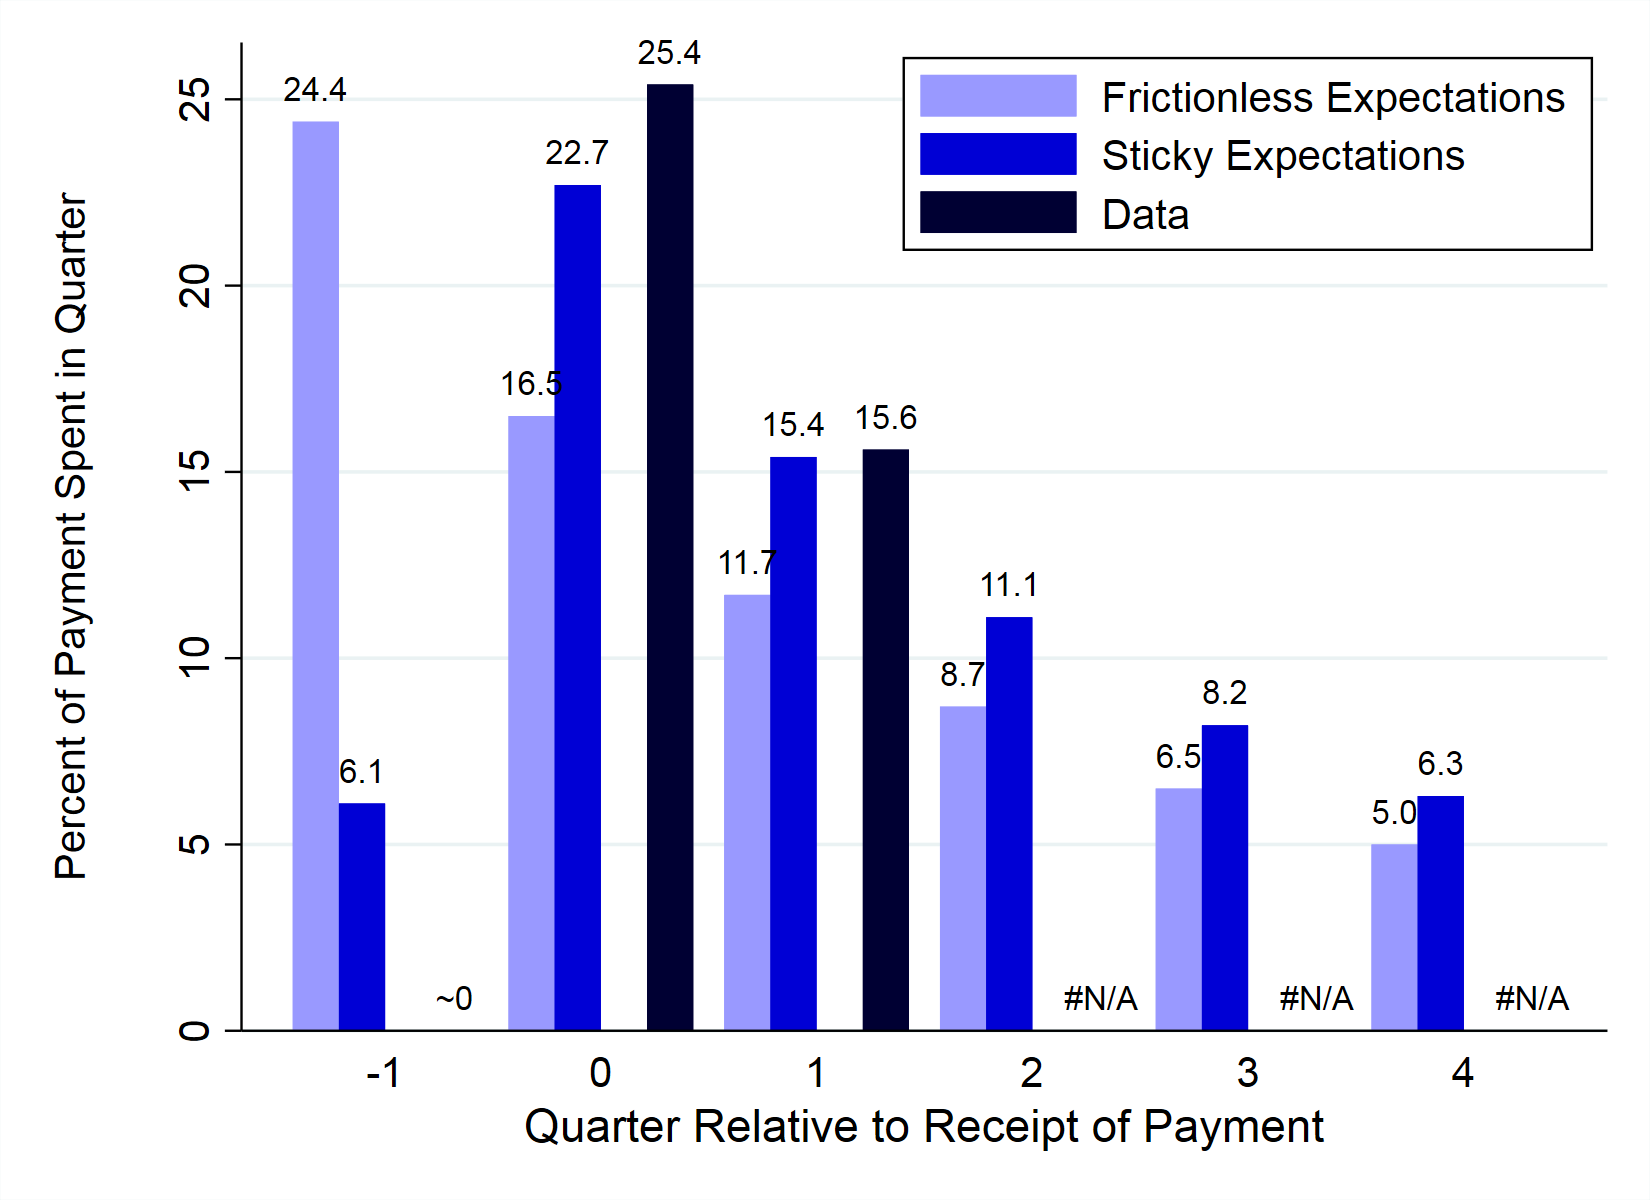
\includegraphics[width=.9\textwidth]{../Figures/parkerExperiment}
	\end{center}
\end{figure}
\end{frame}

\begin{frame}
\frametitle{Conclusion}
\jbemph{
Model with `Sticky Expectations' of aggregate variables can match both micro and macro consumption dynamics}

\begin{eqnarray}
\ifnumSw\Delta \log \mathbf{C}_{t+1} & \approx & \varsigma+\chi \Delta \log \mathbf{C}_{t}+\eta \Ex_{t}[\Delta \log \mathbf{Y}_{t+1}]+\alpha A_{t}+\epsilon_{t+1} \nonumber
\end{eqnarray}

\begin{center}
\begin{tabular}{llccc}
\toprule
        &        & $\chi$       & $\eta$          & $\alpha$
\\ \midrule \multicolumn{2}{l}{Micro }

\\        & Data                   & $\approx 0  $      & $0 < \eta < 1 $ & $< 0$
\\    & Theory: Habits                &  $\approx 0.75$       & $0 < \eta < 1 $ & $< 0$
\\        & Theory: Sticky Expectations                  & $\approx 0  $      & $0 < \eta < 1 $ & $< 0$
\\ \midrule \multicolumn{2}{l}{Macro}
\\ & Data             & $\approx 0.75$     & $\approx 0$           & $< 0$
\\ & Theory: Habits             & $\approx 0.75$     & $\approx 0$           & $< 0$
\\ & Theory: Sticky Expectations             & $\approx 0.75$     & $\approx 0$           & $< 0$
\\ \bottomrule
%\\ & Data:CampMan            &                    & $0.50$                  & $> 0$
%\\ & Data (Sommer)           & $0.7$              & $0.15$                  & $> 0$
%\\ Habits  & $\approx 0.75 $    & $\approx 0$           & $ > 0        $
\end{tabular}
\end{center}

\end{frame}

\tiny

\beamerdefaultoverlayspecification{<*>}

\begin{frame}[t,allowframebreaks,noframenumbering]
\frametitle{References}

%\input econtexBibMake

%\write18{if [ `kpsewhich economics.bib` != '' ]; then touch economics.bib    ; fi} # This should be done only for final versions AFTER bibexport has occurred and \jobname.bib is populated
%\write18{if [ ! -f \jobname.bib     ]; then touch \jobname.bib     ; fi}
%\write18{if [ ! -f \jobname-Add.bib ]; then touch \jobname-Add.bib ; fi}

\bibliographystyle{econtex}
\bibliography{economics,cAndCwithStickyE-Slides,cAndCwithStickyE-Slides-Add}

\end{frame}

\normalsize

\begin{frame}[noframenumbering]
\frametitle{Calibration I}
\label{calibration1}
%\ptsize{9}
\small
\input ../Tables/Calibration_1.tex

\hyperlink{key_parameters}{\beamerbutton{Back}}

\end{frame}

\begin{frame}[noframenumbering]
\frametitle{Calibration II}
%\ptsize{9}
\small
\input ../Tables/Calibration_2.tex

\hyperlink{key_parameters}{\beamerbutton{Back}}
\end{frame}

\begin{frame}[noframenumbering]
  \frametitle{Markov Process for Aggregate Productivity Growth $\Phi$}

$
\pmb{\ell}_{t,i} = \theta_{t,i}\Theta p_{t,i} {P}_{t},\quad
p_{t+1,i} =  {{p}}_{t,i} \psi_{t+1,i},  \quad
 {P}_{t+1} =  \PtyGro_{t+1} {P}_{t}\Psi_{t+1}
$
\bi
\item $\Phi_t$ follows bounded (discrete) RW
\item 11 states; average persistence 2 quarters
\item Flexible way to match actual pty growth data
\ei
  \begin{figure}
\begin{center}
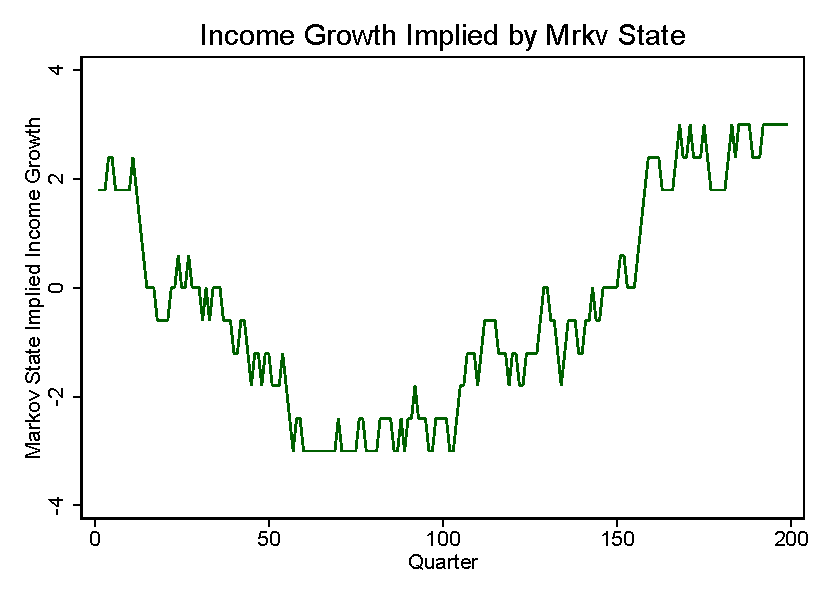
\includegraphics[width=.75\textwidth]{../Figures/MrkvStateGrowth}
\end{center}
\end{figure}

\end{frame}

\begin{frame}[noframenumbering]
\frametitle{Equilibrium}

\footnotesize
\input ../Tables/EqbmSlides.tex

\end{frame}

\begin{comment}
\begin{frame}[noframenumbering]
\frametitle{Cost of Stickiness}
Define (for given parameter values):
\begin{center}
\begin{tabular}{rl}
${v}(\Wage_t,\cdot)$ & Newborns' expected value for frictionless model
\\ $\grave{v}(\Wage,\cdot)$ & Newborns' expected value if $\sigma^{2}_{\psi}=0$
\\ $\perc{v}(\Wage,\cdot)$ & Newborns' expected value from sticky behavior
\end{tabular}
\end{center}

Fact suggested by theory (and confirmed numerically):
\input \eq/vApprox.tex

Guess (and verify) that:
\input \eq/vApproxSticky.tex

\end{frame}

\begin{frame}[noframenumbering]
\frametitle{Cost of Stickiness: $\omega$ and $\Pi$}

Costs of stickiness $\omega$ and prob of aggr info updating $\Pi$

\begin{figure}
\label{costOfStickiness}
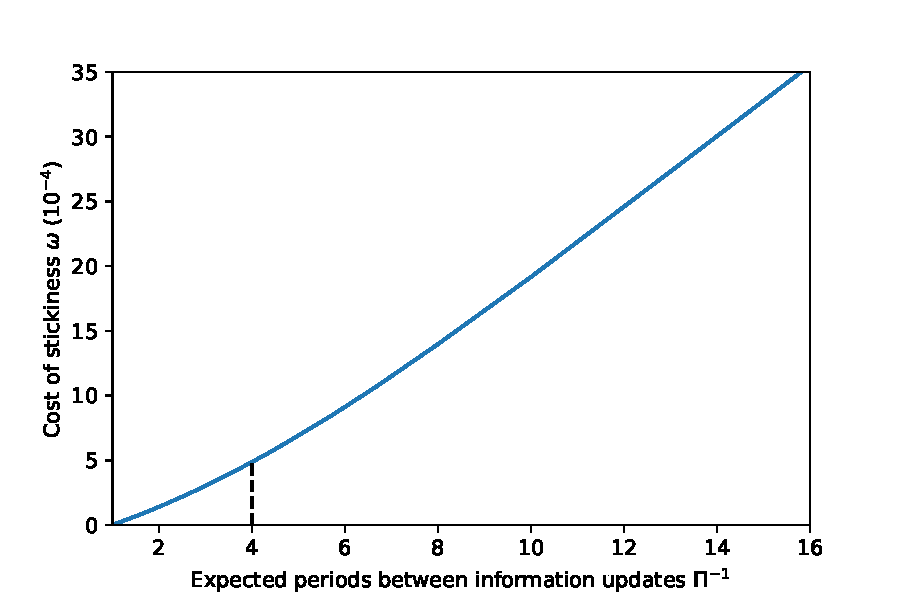
\includegraphics[width=0.9\textwidth, height=6cm]{../Figures/uCostvsPiInv.pdf}\\
\tiny Notes: The figure shows how the utility costs of updating $\omega$ depend on the probability of updating of aggregate information $\Pi$ in the SOE model.
\end{figure}

\end{frame}

\begin{frame}[noframenumbering]
\frametitle{Cost of Stickiness: Solution}
Suppose utility cost of attention is $\iota\Pi$.
\begin{itemize}
\item If Newborns Pick Optimal $\Pi$, they solve
\end{itemize}

\input \eq/pickPi.tex

Solution:
\input \eq/bestPi.tex

Optimal $\Pi$ characteristics:
\begin{itemize}
\item Increasing in $\kappa$ (`importance' to value of perm shocks)
\item Increasing in $\sigma_{\psi}$ (`magnitude' of perm shocks)
\item Decreasing as attention becomes more costly: $\iota \uparrow$
\end{itemize}

\end{frame}
\end{comment}

\begin{frame}[noframenumbering]
\frametitle{Is Muth--Lucas--Pischke Kalman Filter Equivalent?}

\jbemph{No.}\\
\cite{muthOptimal}--\cite{lucas:imperfectInfo}--\cite{pischkeMicroMacro} Kalman filter
\begin{itemize}
\item  All you can see is Y
\begin{itemize}
\item Lucas: Can't distinguish agg. from idio.
\item Muth--Pischke: Can't distinguish tran from perm
\end{itemize}

\item Here: Can see own circumstances perfectly

\item Only the (tiny) aggregate part is hard to see

\item \jbemph{Signal extraction for aggregate $\mathbf{Y}_t$ gives too little persistence in $\Delta \mathbf{C}_t$: $\chi\approx 0.17$}

\end{itemize}

\end{frame}

\begin{frame}[noframenumbering]
\frametitle{Muth--Pischke Perception Dynamics}

\begin{itemize}
\item Optimal signal extraction problem (Kalman filter):\\
Observe $\mathbf{Y}$ (aggregate income), estimate $P$, $\Theta$
\item Optimal estimate of ${P}$:
\begin{eqnarray*}
   \ifnumSw  \hat{{P}}_{t+1} & = & \Pi \mathbf{Y}_{t+1} + (1-\Pi) \hat{{P}}_{t},
\end{eqnarray*}
where for signal-to-noise ratio $\varphi = \sigma_{\PShk}/\sigma_{\Theta}$:
\input \eq/SigToNoise.tex
\item But if we calibrate $\varphi$ using observed macro data
  \begin{itemize}

\item \jbemph{$\Rightarrow \Delta \log \mathbf{C}_{t+1} \approx $ 0.17 $ \Delta \log \mathbf{C}_{t}$}
\item \jbemph{Too little persistence!
}
\end{itemize}
\end{itemize}

\end{frame}

\end{document}
